% Informe de Proyecto % Autor: Tu Nombre % Fecha: Fecha actual

\documentclass[11pt,a4paper]{article}

\usepackage[spanish]{babel} 
\usepackage[utf8]{inputenc} 
\usepackage{graphicx}
\usepackage{hyperref}

\title{Actas Capitulares de la Habana} \author{Edian Broche Castro \\ Roger Fuentes Rodr\'iguez \\ Kevin Manzano Rodr\'iguez \\ Massiel Paz Otaño \\ Jackson Claudio Vera Pineda} \date{}

\begin{document}

\maketitle

\tableofcontents

\section{Introducción}
\subsection{Objetivo del Proyecto} 

Se tiene como objetivo desarrollar una propuesta de transcripción y procesamiento de un conjunto de imágenes, para su posterior uso como dataset en futuros proyectos para identificar entidades nombradas y crear grafos de conocimiento.  

\subsection{Contexto}

Se tiene una serie documental perteneciente al fondo Ayuntamiento de La Habana del Archivo Histórico de la Oficina del Historiador de la Ciudad de la Habana.

Esta serie documental se divide en dos grupos o subseries: los libros originales (1550 - 1898) y los libros trasuntados (1550 - 1809). Los primeros destacan por su riqueza de contenido y forma; los segundos por dejar constancia de la labor del Ayuntamiento para garantizar la perdurabilidad en el tiempo de este tipo documental, al ser copias realizadas en la segunda mitad del siglo XIX.

Las actas dejan la huella de una institución colonial y su devenir en el tiempo: el Ayuntamiento. Ellas recogen los planteamientos y discusiones de aquellos problemas que interesaron a los pobladores del lugar, ya fueran de índole económica, política o social; están reflejados los hechos más significativos de cada una de las épocas.

Se tiene como corpus el tomo 1 digitalizado, el resto está en proceso de digitalización.

\section{Metodología} 
\subsection{Enfoque del Proyecto} 

Existen m\'ultiples herramientas para la transcripción de documentos hist\'oricos entre estas destacan \href{https://www.transkribus.org/}{Transkribus} la cual fue recomendada por el cliente por su uso en anteriores trabajos, pero debido al deterioro de los documentos adem\'as del tipo espec\'ifico de tipograf\'ia los resultados no eran satisfactorios. Debido al bajo \textbf{accuracy} provisto por esta herramienta creada por especialistas en el tema podemos asumir que el problema es bastante complejo.

\begin{center} 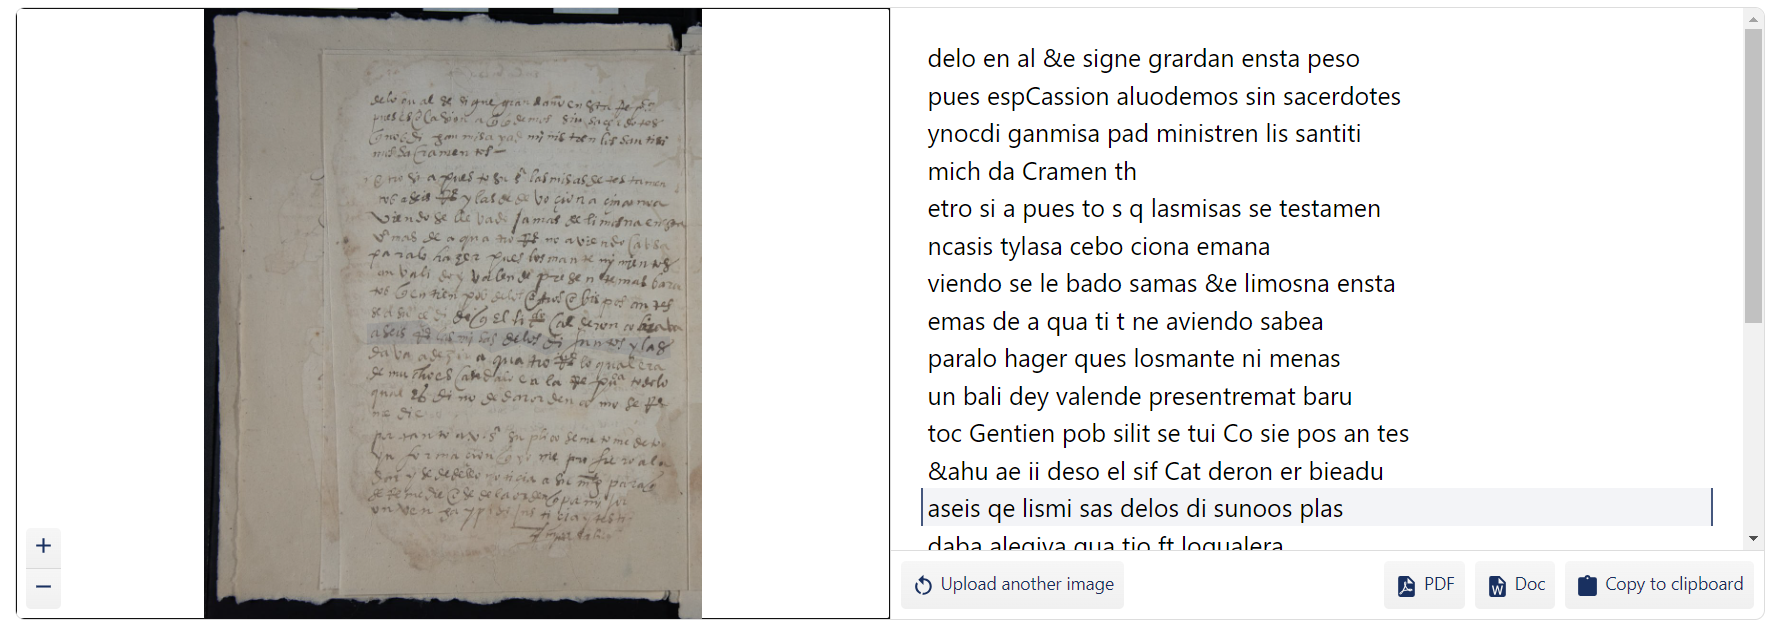
\includegraphics[width=1.0\textwidth]{transkribus} \end{center}

Nos encontramos con dos grandes problemas: falta de datos para llevar a cabo el entrenamiento de alg\'un modelo, pues muchos de los datasets encontrados no poseen el idioma requerido (Español) ni el tipo de letra (procesal-cortesana); y una tarea que solo un ojo humano especializado podr\'ia realizar (tip\'ografo)

Debido a todo lo expuesto, el proyecto fue enfocado en una b\'usqueda exhaustiva de datos clasificados, un procesamiento minucioso de las im\'agenes, el uso de varios OCRs, y un posprocesamiento con diccionarios del idioma y LLM.

\subsection{Recursos Utilizados}

Como lenguaje principal se utilizó Python, debido a que brinda un f\'acil acceso a bibliotecas de procesamiento de texto e im\'agenes. Entre las utilizadas destacan: \textbf{Kraken}, \textbf{PIL}, \textbf{TensorFlow}, \textbf{Numpy}, \textbf{matplotlib}, \textbf{scipy}, \textbf{spacy}, \textbf{symspellpy}, \textbf{transformers}, \textbf{cv2}, \textbf{sam2}.

El LLM utilizado fue \textbf{Gemini} por cuestiones económicas, y como diccionario de frequencias, \href{https://github.com/hermitdave/FrequencyWords/blob/master/content/2016/es/es_full.txt}{spanish frequency dictionary} (se consideró la creaci\'on de un diccionario a partir de un libro escrito por Luis XV, pero se tendr\'ian muy pocas palabras en comparaci\'on con el utilizado). El modelo de spacy empleado fue \textbf{es core news sm}.

Entre los datos recopilados inicialmente se utiliz\'o \href{https://zenodo.org/records/1490009/files/Rodrigo%20corpus%201.0.0.tar.gz?download=1}{dataset de rodrigo}. Este, es un dataset de Español antiguo, pero la tipograf\'ia no coincide, pues en este caso se utiliza letra g\'otica y nuestro (se necesita que sea procesal-cortesana). Luego, se encontr\'o todo un corpus de documentos en Español de años anteriores a 1900: \href{https://corpuscodea.es/}{CODEA} y con una estructura que se puede aprovechar. La mayor\'ia de los documentos presentan una triple representaci\'on: la imagen, una transcripción paleogr\'afica, y una presentanci\'on cr\'itica. El dataset inicialmente tiene alrededor de 4000 documentos, pero luego de filtrar por el tipo de letra requerida se reduce a 546, recalcando la dificultad de los datos.\\

AQUI FALTAN AGREGAR COSAS (resultado de cada OCR)\\

\section{Resultados} 
\subsection{Logros Principales} 

En la primera etapa del producto se logra una mejora considerable en la imagen, haciendo uso de un pipeline para limpiar las im\'agenes, llev\'andola a escala de grises, y aplicando t\'ecnicas de filtrado como filtro Gaussiano, para disminuir el ruido general de la imagen, ecualización de histograma para mejorar el contraste de la imagen y resaltar la letra en los documentos, y operaciones morfológicas de erosión y dilatación para mejorar el trazo en los documentos. Finalizando con una binarización de la biblioteca \textit{Kraken}, con modelos basados en redes neuronales profundas y binarización adaptativa, y entrenados con documentos históricos. La figura \ref{fig:tresfotosmodelo} muestra el resultado de una foto pasando por las etapas claves del procesamiento.\\

Para el tratado de las manchas debido a la longevidad de los documentos(son amarillos) se implement\'o un conversor personalizado de la imagen de color a escala de grises, ponderando las componentes rgb de forma diferente a lo usual (que es el promedio);$r + g$ es el equivalente al amarillo por lo que se ponderó $r$ y $g$ en menor grado variando los par\'ametros para tratar de contrarrestar el ruido.

\begin{figure}[h] \centering \begin{minipage}{1.0\textwidth} 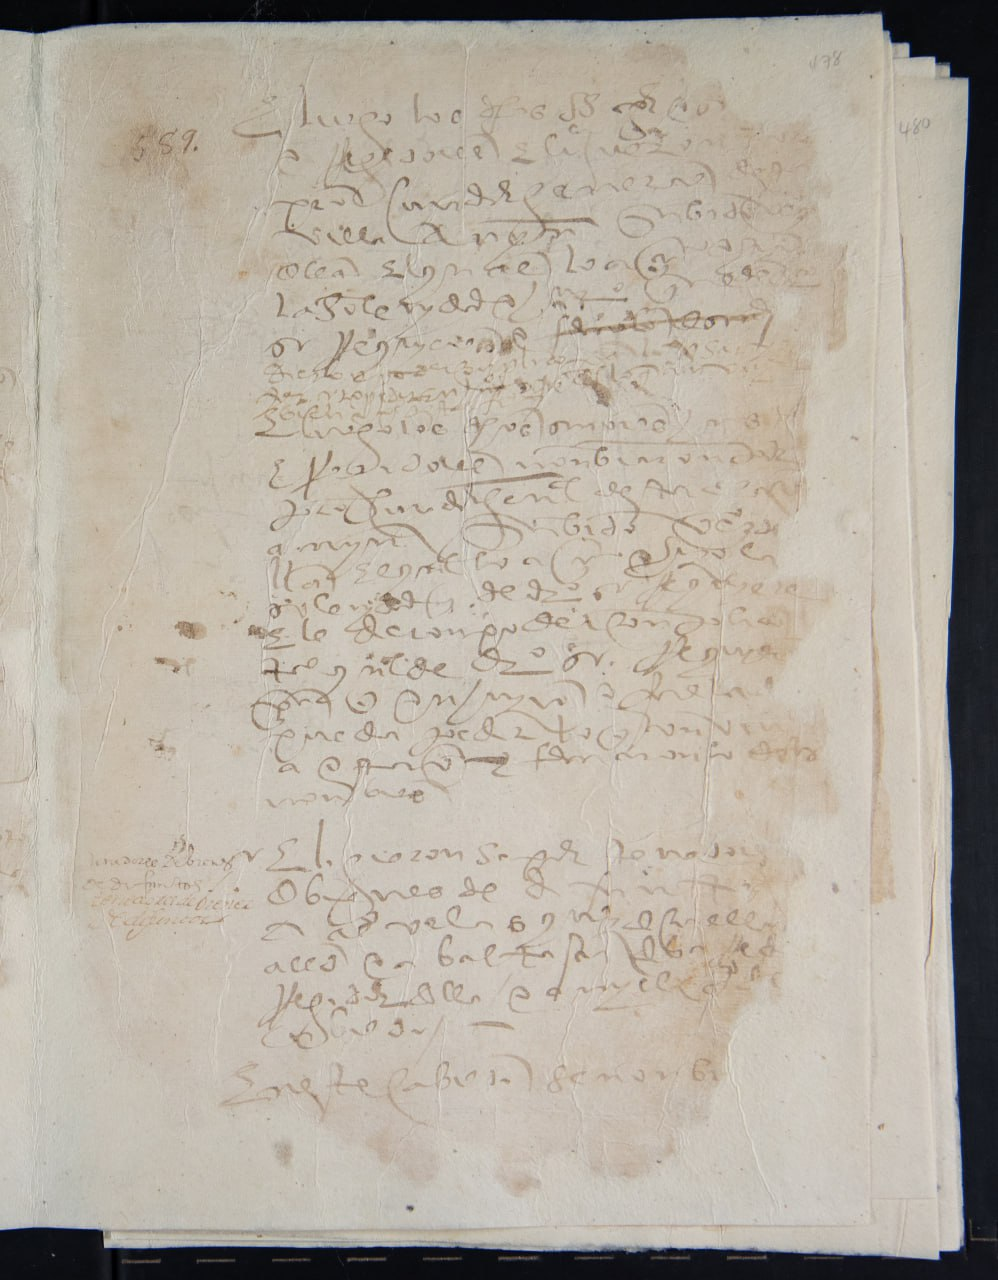
\includegraphics[width=0.32\textwidth]{original.jpg} 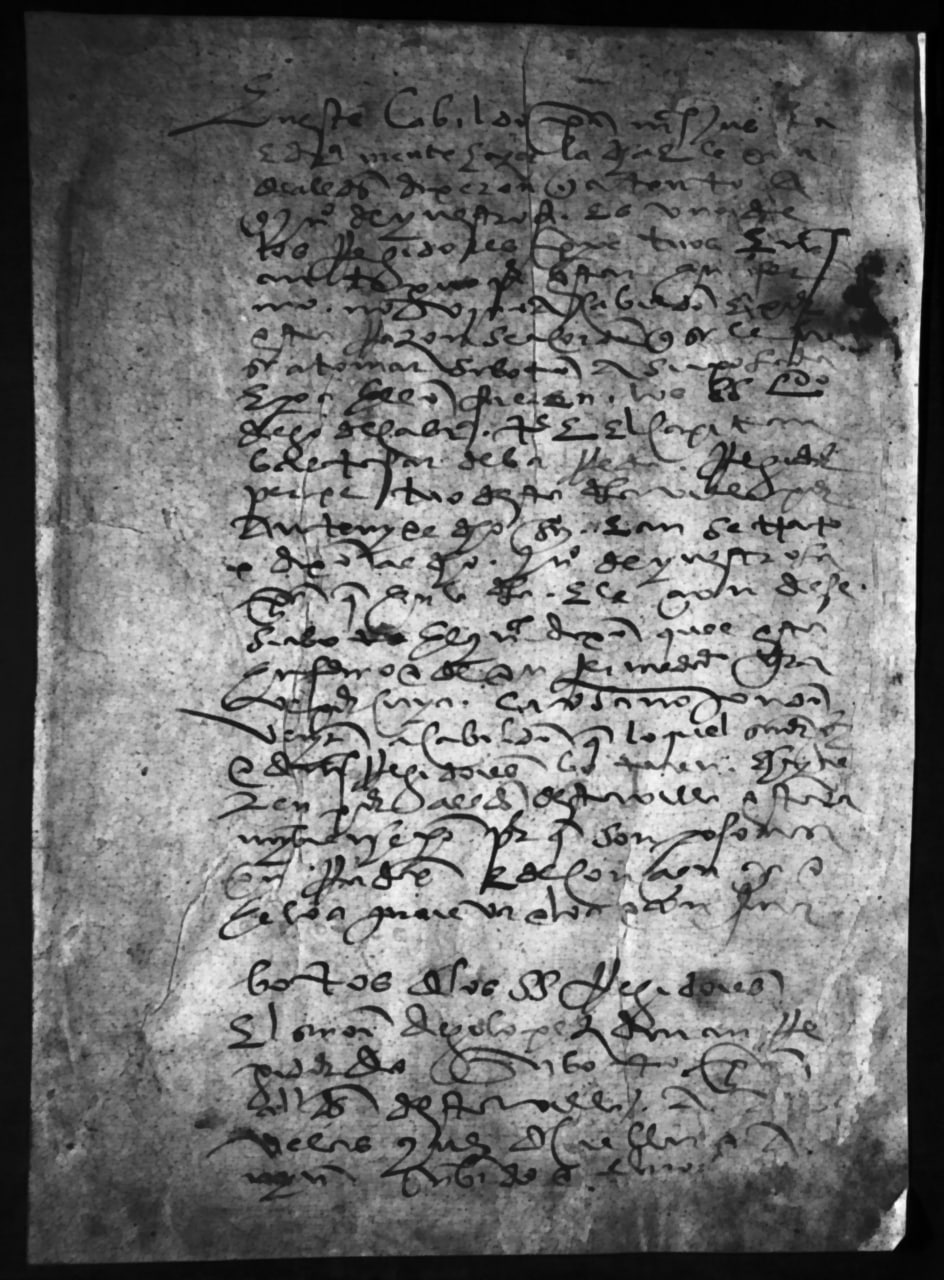
\includegraphics[width=0.32\textwidth]{morph.jpg} 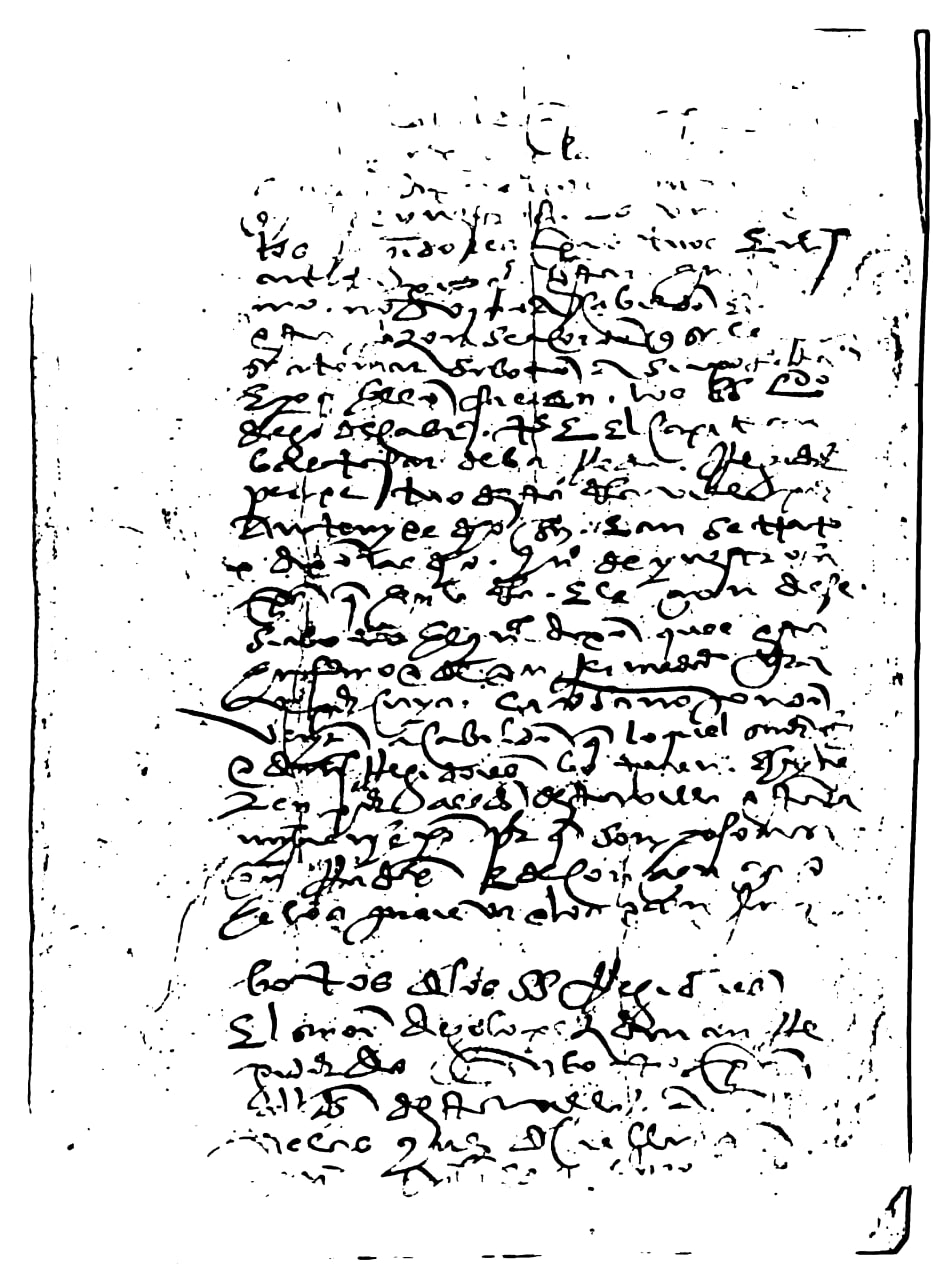
\includegraphics[width=0.32\textwidth]{kraken.jpg} \caption{Original, en escala de grises con letra reconstruida, imagen binarizada} \label{fig:tresfotosmodelo} \end{minipage} \end{figure}

Por otra parte, se intentó el uso de algoritmos de detecci\'on de bordes como \textit{sobel}, \textit{Canny}, y \textit{laplaciano} , el \'ultimo no funcionó bien porque depende de la segunda derivada de los cambios pixel a pixel, y esto en documentos de texto, donde el documento es blanco y las letras son negras, sumado a que los cambios de papel tinta son muy abruptos, indefine la derivada y causó malos resultados. En los otros dos casos el ajuste fue aceptable en algunos casos como se muestra en la figura \ref{fig:tresfotos}, pero no así en la mayoría de los documentos.\\

\begin{figure}[h] \centering \begin{minipage}{1.0\textwidth} 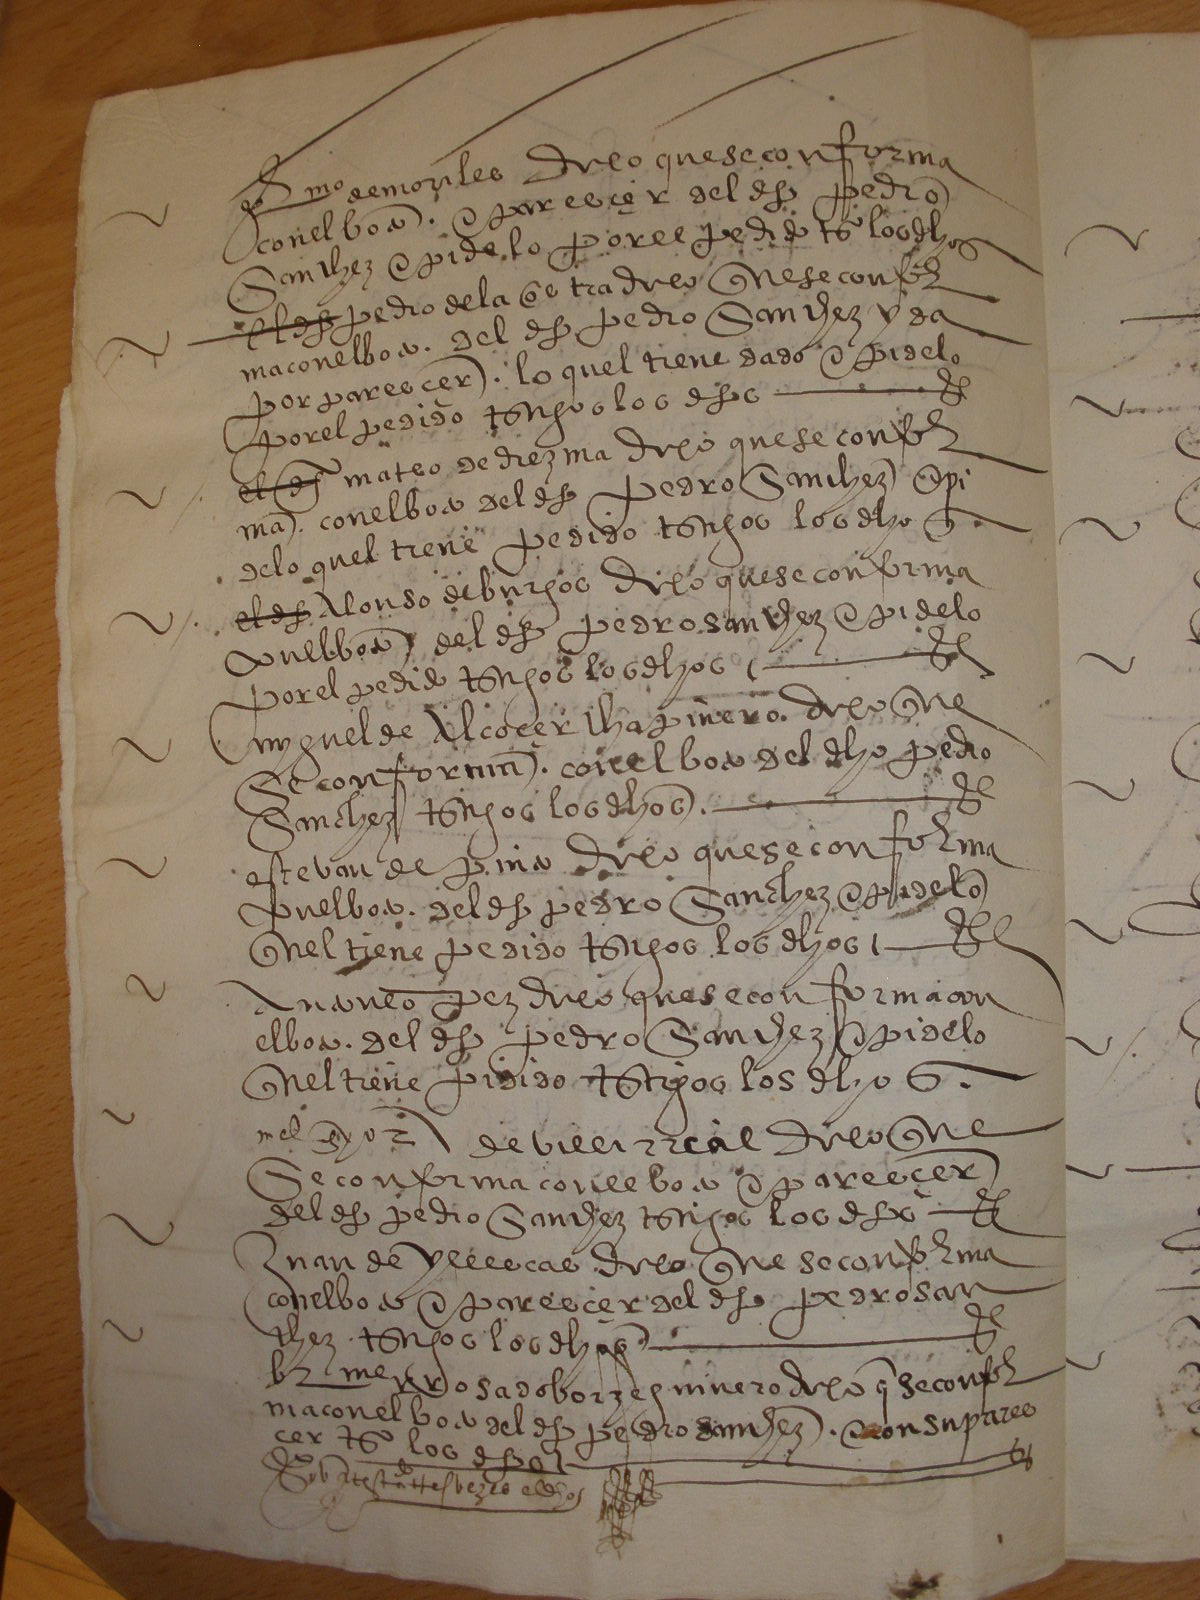
\includegraphics[width=0.32\textwidth]{CODEA-0205_2v.jpg} 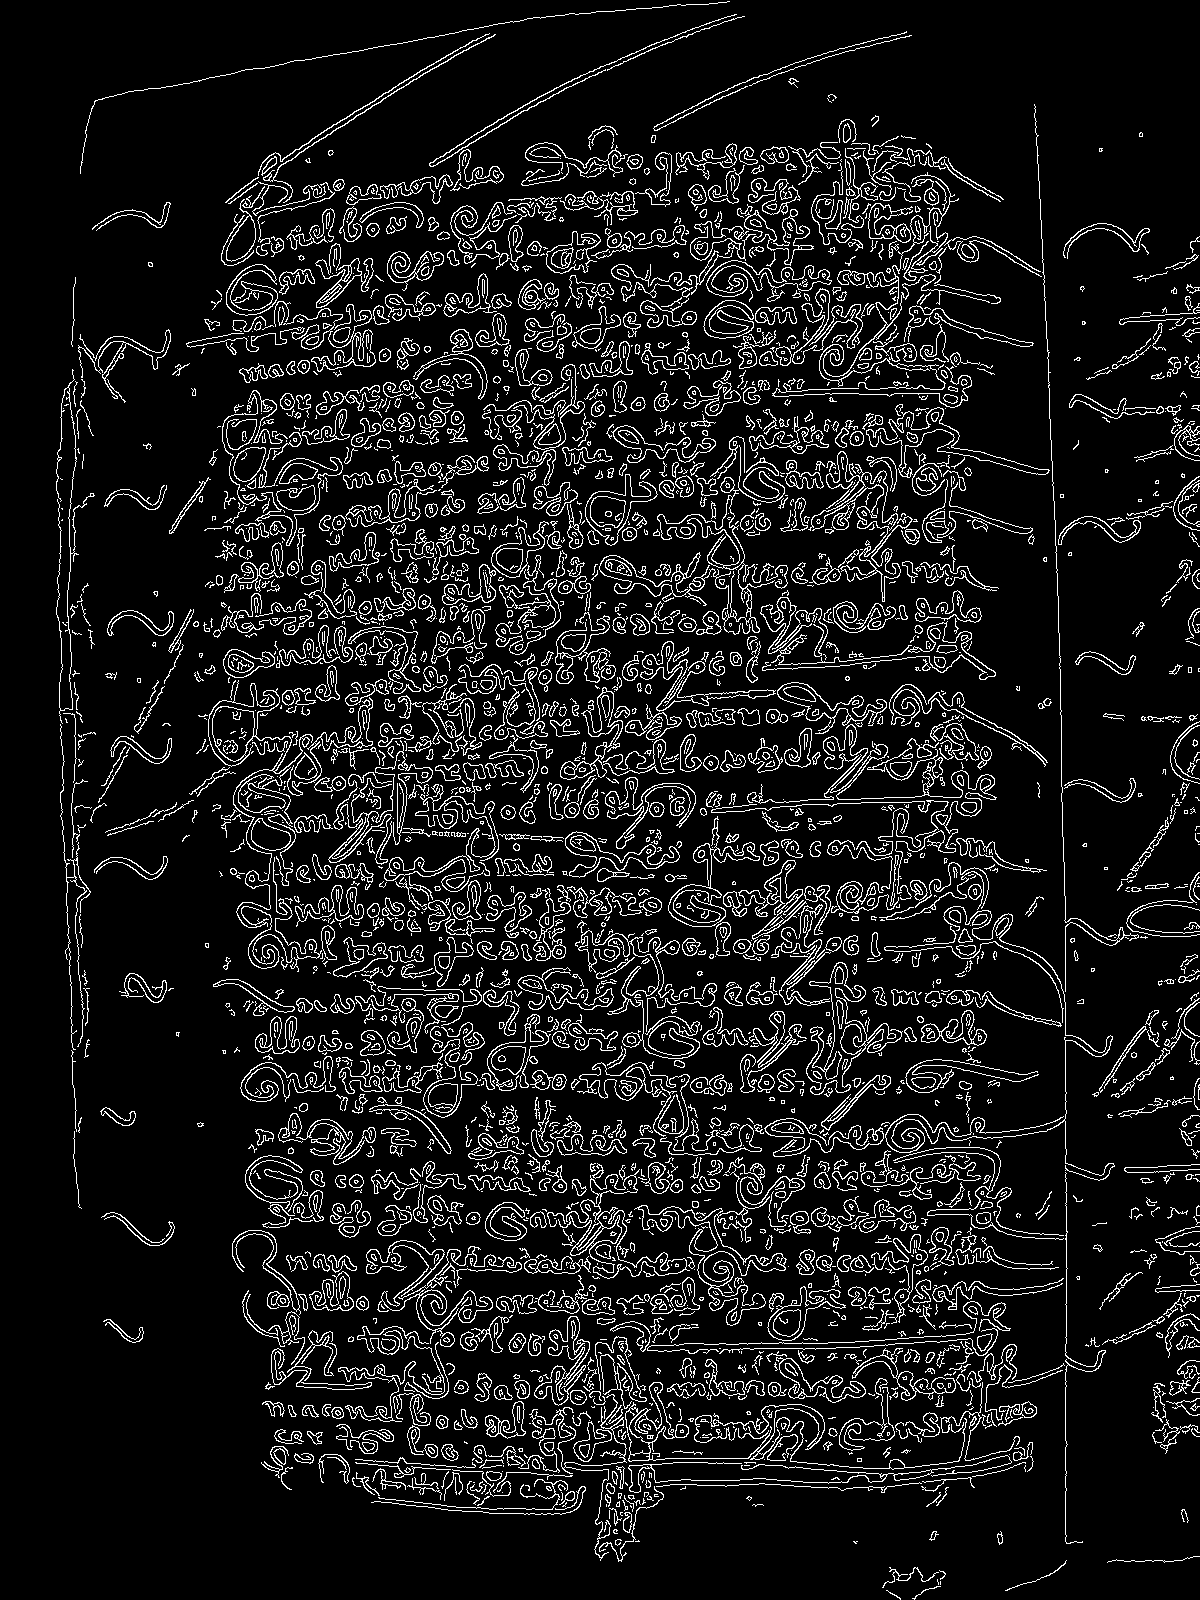
\includegraphics[width=0.32\textwidth]{canny_image_aftergauss_eq2.png} 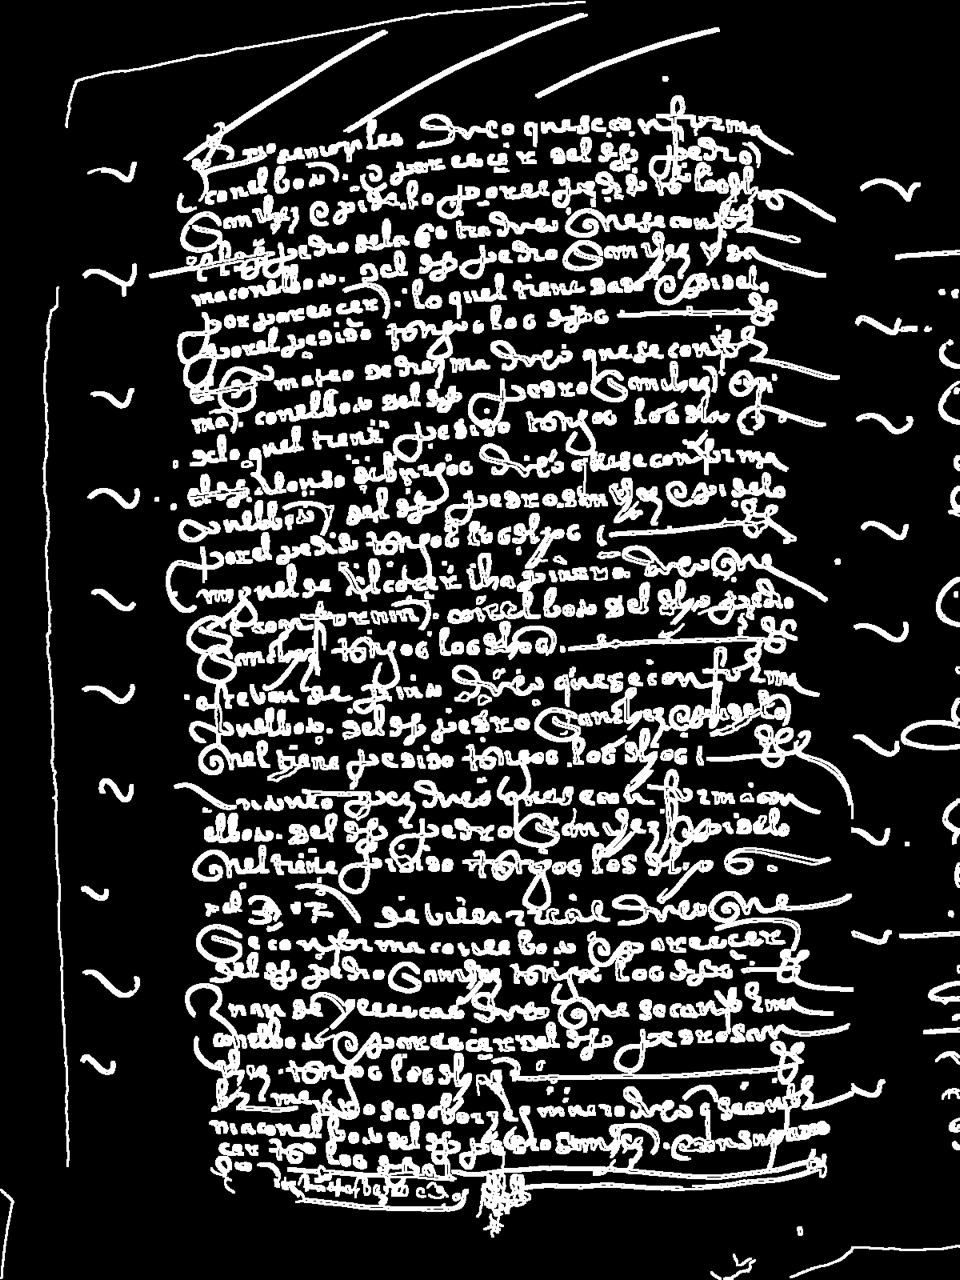
\includegraphics[width=0.32\textwidth]{photo_2025-01-27_21-34-01.jpg} \caption{Original, detecci\'on de bordes, operaciones morfol\'ogicas de izquieda a derecha} \label{fig:tresfotos} \end{minipage} \end{figure}

Se intent\'o adem\'as el uso de filtros de mediana, para aminorar el ruido \textit{sal y pimienta}, as\'i como filtro bilateral, sin mejor\'ias significativas en los resultados. Se probó la binarizaci\'on de la imagen, definiendo un umbral de intensidad donde si $x > threshold$ se toma como letra y en caso contrario como fondo, pero en zonas de sombra, probando con diferentes valores para threshold no se detecta bien la escritura, tambi\'en se intentó binarizaci\'on adaptativa convencional pero se recuperaba mucho ruido y manchas en el documento.\\


Luego de binarizadas las im\'agenes son pasadas por dos procesos de segmentación, uno que brinda \textbf{Kraken} y una proyecci\'on de histogramas (se sugiere utilizar la primera pues otorga mejores resultados), y en caso de un proceso manual ser\'ia mejor utilizar \textbf{SAM2}, pero no logramos automatizar el proceso. Sin embargo, esta última herramienta, aunque poderosa, no ofrece resultados tan satisfactorios, pues en el momento de encerrar manualmente en \textit{cajas} a cada línea del documento, es necesario que estas (las líneas) sean lo más rectas posibles; lo cual se hace complejo de encontrar dado que se trata de documentos manuscritos. \\
Luego de segmentada la imagen, esta es pasada a 3 OCRs distintos: \textbf{SimpleHTR}, \textbf{sinai-sam-rec-v4-best}, \textbf{McCATMuS-nfd-nofix-V1}, los cuales son modelos especializados en \textbf{handrwitten recognition}. Los dos \'ultimos provienen de Kraken. Cada uno tuvo que tratarse de forma diferente dado que el primero necesita la imagen segmentada, y los otros solamente los \textbf{bounding box}.\\

En la \'ultima etapa, una vez procesadas la im\'agenes con las t\'ecnicas para mejorarlas y extraído el texto con los diferentes OCRs, se realiz\'o un posprocesamiento para mejorar la calidad de las transcripciones. Inspirados en el DataSet de CODEA, se brindó una transcripción cr\'itica del documento. Dada la naturaleza de los documentos y los errores inherentes al OCR, implementamos un pipeline para corregir errores ortogr\'aficos y ajustar la chorencia del texto, refinando la salida.\\

Se utiliz\'o un modelo de lenguaje \textbf{Spacy} para segmentar el texto en tokens, para as\'i identificar palabras y elementos no alfab\'eticos. Cada token fue corregido utilizando \textit{SymSpell}, una herramienta basada en un diccionario de frecuencias, para separar correctamente palabras unidas y capitalizarlas. Tras  las correcciones, se utiliz\'o un modelo generativo, \textit{Gemini} para realizar un refinamiento sem\'antico y estil\'istico, corrigiendo as\'i el formato del texto y la gram\'atica, adem\'as de mantener el contexto hist\'orico del español antiguio. Tambi\'en se consideraron las diferentes salidas y se combinaron en una sola.\\

A continuaci\'on un ejemplo del flujo:

\begin{enumerate}
    \item Essta es una prueva de ectraccion de teexto. Connoscida cosa sea a todos los queesta carta uieren como yo don Fferrando por la gracia de dios hey de Castiella
    \item Esta es una prueba de extracción de texto. Conocida cosa sea a todos los que esta carta vieren como yo don Fferrando por la gracia de Dios hay de Castilla
    \item Esta es una prueba de extracción de texto. Conocida cosa sea a todos aquellos que esta carta vieran, como yo, don Fernando, por la gracia de Dios, rey de Castilla.
\end{enumerate}

\subsection{Desafíos Superados}

En el momento de la segmentación jug\'o un papel fundamental la b\'usqueda de par\'ametros adecuados para que tuviera mejor rendimiento los procesos posteriores.\\

Entre los desaf\'ios superados en el posprocesamiento nos encontramos con la conservaci\'on del español antiguo, pues no hallamos un diccionario de frecuencias de esa época; sin embargo, solventamos este problema con el LLM utilizado, la obtención del mismo fue compleja, pues se probaron con otros, por ejemplo: \textbf{GPT-2}, \textbf{"google/mt5-small"}, \textbf{flax-community/spanish-t5-small}, pero los resultados fueron p\'esimos en los tres casos, adem\'as de que no ten\'iamos un API c\'omoda y los modelos eran bastantes pesados, por lo que optamos por \textbf{Gemini}.

\section{Conclusiones} 
\subsection{Impacto del Proyecto} 

El proyecto planea ser utilizado para la transcripción de documentos hist\'oricos archivados en la oficina del historiador, inicialmente se tiene un solo tomo, pero luego de terminar el proceso de digitalizaci\'on de los siguientes tomos ya se podr\'a directamente pasar a transcripci\'on para su posterior an\'alisis. También puede utilizarse el resultado del mismo para convertirlo en producto reutilizable con el objetivo de crear alguna herramienta para encontrar entidades, y poder realizar búsqueda de interés, para encontrar información valiosa en estos documentos. 

\subsection{Recomendaciones para Futuras Implementaciones}
Se recomienda indagar sobre la posibilidad de usar el algoritmo \textit{DBSCAN} para la segmentación en este tipo de documentos, debido a la naturaleza curva e irregular de las líneas en documentos manuscritos con tipografía\textit{procesal-cortesana}. Luego, seguir utilizando \textbf{SimpleHTR}, pero se recomienda tener un dataset para hacerle un \textbf{fine tunning} al igual que al modelo generativo que no es espec\'ificamente para esta tarea. Se pudiera volver a utilizar \textbf{GPT-2} pero entrenado en esta cuesti\'on y debería de obtener buenos resultados.

\bibliographystyle{plain} 
\bibliography{referencias}

\begin{thebibliography}{9}

    \bibitem{Avila2020corpus}
    Vicente Marcet Rodriguez
    \textit{El copus de documentos de \'Avila del Hispanic Museum and Library (siglos XV y XVI). Descripci\'on y an\'alisis paleogr\'afico y gr\'afico-fonol\'ogico.}

    \bibitem{granet2018transfer}
    A. Granet, E. Morin, H. Mouchère, S. Quiniou, y C. Viard-Gaudin, 
    \textit{Transfer Learning for Handwriting Recognition on Historical Documents}, 
    ICPRAM, 2018.
    
    \bibitem{torres2025htr}
    S. Torres Aguilar, 
    \textit{Handwritten Text Recognition for Historical Documents using Visual Language Models and GANs}, 
    ArXiv, 2025.
    
    \bibitem{granell2018transcription}
    E. Granell, E. Chammas, L. Likforman-Sulem, C. D. Martínez-Hinarejos, C. Mokbel, y B. I. Cîrstea, 
    \textit{Transcription of Spanish Historical Handwritten Documents with Deep Neural Networks}, 
    Journal of Imaging, vol. 4, no. 15, 2018.
    
    \bibitem{survey_post_ocr}
    THI TUYET HAI NGUYEN, ADAM JATOWT, MICKAEL COUSTATY and ANTOINE DOUCET
    \textit{Survey of Post-OCR Processing Approaches}, 
    2025.

    \bibitem{LightweightOCR}
    Yuning Du, Chenxia Li, Ruoyu Guo, Xiaoting Yin, Weiwei Liu,
Jun Zhou, Yifan Bai, Zilin Yu, Yehua Yang, Qingqing Dang, Haoshuang Wang
    \textit{PP-OCR: A Practical Ultra Lightweight OCR System}
    
    \bibitem{IJARSCT2023extraction}
    Prof. Anuradha Thorat, Mayur Zagade, Shivani More, Manish Pasalkar, Anand Narute
    \textit{Research Paper on Text Extraction using OCR}, 
    IJARSCT, Volume 3, Issue 14, May 2023

    \bibitem{IJIREM2022extraction}
    Ojas Kumar Barawal, and Dr Yojna Arora
    \textit{Text Extraction from Image }, 
    IJIREM, Volume 9, Issue 3, May 2022

\end{thebibliography}


\end{document} $